
%-------------------------------------------------------------
%       WIDGET ORIGINI
%-------------------------------------------------------------

\mcchap{Widgets di Kirivo}{cap:w-k}


%-------------------------------------------------------------
%       WIDGET KIRIVO
%-------------------------------------------------------------

\newpage

% ---------------- Kirivo - Immagini Speciali ----------------

\section{Kirivo - Immagini Speciali}

Il Widget "Kirivo - Immagini Speciali" permette di modificare il contenuto
delle prime due immagini della Homepage, ovvero le immagini solitamente dedicate
allo speciale del mese e alle offerte 

I campi che si possono modificare sono (riferirsi a Figure \ref{fig:kspec}):
\begin{itemize}
\item Link speciale: l'URL dove si viene indirizzati quando si schiaccia sull'immagine dello speciale
\item Url immagine speciale desktop: l'url dell'immagine da mettere nello speciale per desktop
\item Url immagine speciale mobile: l'url dell'immagine da mettere nello speciale per mobile
\item Link offerte: l'URL dove si viene indirizzati quando si schiaccia sull'immagine delle offerte
\item Url offerte speciale desktop: l'url dell'immagine da mettere nelle offerte per desktop
\item Url offerte speciale mobile: l'url dell'immagine da mettere nelle offerte per mobile
\end{itemize}

\begin{figure}
  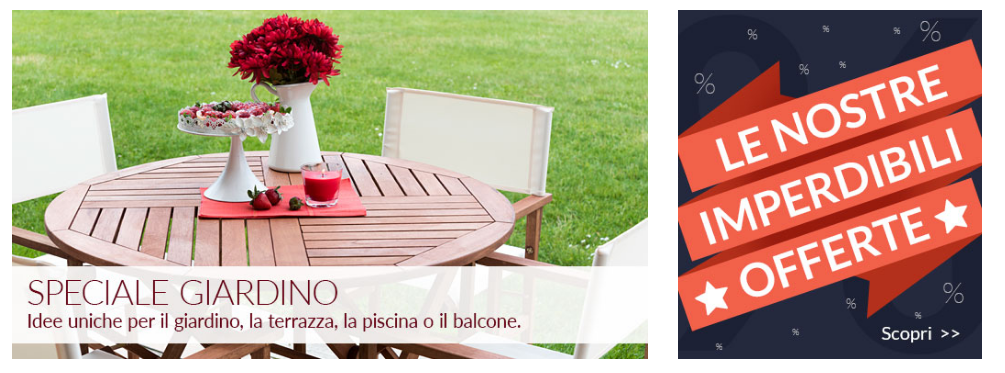
\includegraphics[width=\textwidth]{figure/kspec.png}
  \caption{Contenuto mostrato dal widget "Kirivo - Immagini Speciali".}
  \label{fig:kspec}
\end{figure}

% ---------------- Kirivo - Immagini Newsletter ----------------

\newpage
\section{Kirivo - Immagini Newsletter}

Il Widget "Kirivo - Immagini Newsletter" permette di modificare il contenuto
delle prime due immagini della Homepage, ovvero le immagini solitamente dedicate
allo speciale del mese e alle offerte 

I campi che si possono modificare sono (riferirsi a Figure \ref{fig:knews}):
\begin{itemize}
\item Url immagine newsletter desktop: l'url dell'immagine da mettere nella sezione "iscriviti alla newsletter"
\item Url immagine newsletter mobile: l'url dell'immagine da mettere nella sezione "iscriviti alla newsletter"
\item Link offerta: l'URL dove si viene indirizzati quando si schiaccia sull'immagine dell'offerta
\item Url offerta desktop: l'url dell'immagine da mettere nelle offerta per desktop
\item Url offerta mobile: l'url dell'immagine da mettere nelle offerta per mobile
\end{itemize}

\begin{figure}
  
\includegraphics[width=\textwidth]{figure/knews.png}
  \caption{Contenuto mostrato dal widget "Kirivo - Immagini Newsletter".}
  \label{fig:knews}
\end{figure}

% ---------------- Kirivo - Prodotti in evidenza ----------------

\newpage
\section{Kirivo - Prodotti in evidenza}

Il Widget "Kirivo - Prodotti in evidenza" visualizza quella porzione di HTML usata
per visualizzare i prodotti in evidenza (vedi Figure \ref{fig:kevid}).

I campi che si possono modificare sono (riferirsi a Figure \ref{fig:kevid}):
\begin{itemize}
\item Titolo: il testo "PRODOTTI IN EVIDENZA".
\item Ids: l'ID dei prodotti da visualizzare separati da virgola. I prodotti devono
essere almeno tre, se sono più di tre verranno usati i primi 3 ID validi.
\end{itemize}

\begin{figure}
  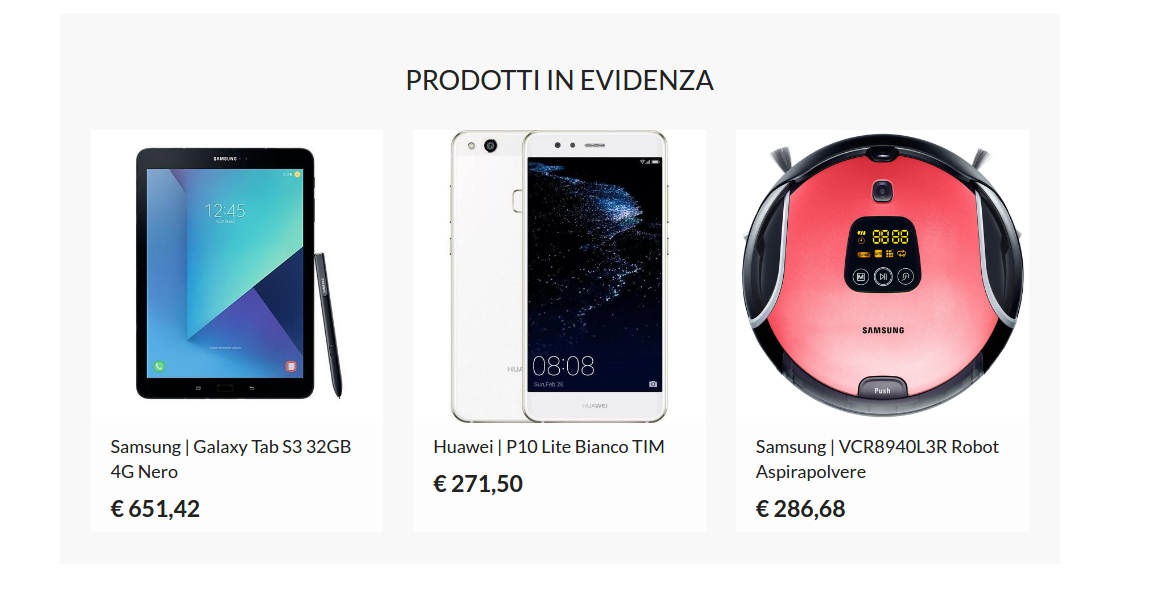
\includegraphics[width=\textwidth]{figure/kevid.png}
  \caption{Contenuto mostrato dal widget "Kirivo - Prodotti in evidenza".}
  \label{fig:kevid}
\end{figure}

\newpage
\section{Kirivo - Slider prodotti}

% ---------------- Kirivo - Slider prodotti ----------------

Il Widget "Kirivo - Slider prodotti"   visualizza quella porzione di HTML usata
per visualizzare uno slider di un insieme di prodotti (vedi Figure \ref{fig:kslide}).

I campi che si possono modificare sono (riferirsi a Figure \ref{fig:kslide}):
\begin{itemize}
\item Titolo: il testo "PRODOTTI PIÙ POPOLARI".
\item Numero max: il numero massimo di prodotti da visualizzare. Se lasciato vuoto non viene imposto alcun limite.
\item Ids: l'ID dei prodotti da visualizzare separati da virgola. I prodotti devono
essere almeno quanti specificati in numero max o quattro se non viene specificato.
\end{itemize}

\begin{figure}
  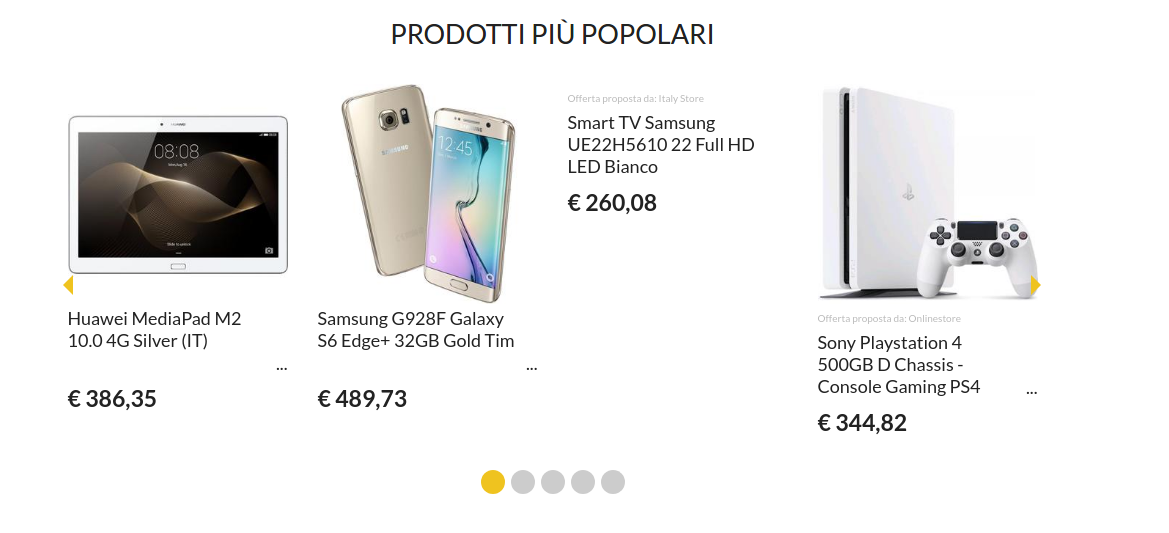
\includegraphics[width=\textwidth]{figure/kslide.png}
  \caption{Contenuto mostrato dal widget "Kirivo - Slider prodotti".}
  \label{fig:kslide}
\end{figure}

